\documentclass[11pt]{article}

\usepackage[margin=1in]{geometry}
\usepackage{amsmath,amssymb}
\usepackage{booktabs}
\usepackage{graphicx}
\usepackage{hyperref}
\usepackage[numbers,sort&compress]{natbib}

\graphicspath{{figures/}{../repro/figures/pam_diagnostics/}{../repro/figures/hardmove/}}

\title{Physics-Aware Mode Reordering for Tensor-Train Policy Iteration}
\author{Anonymous Authors}
\date{}

\begin{document}
\maketitle

\begin{abstract}
This draft is a repository-synchronized working manuscript. Claims, numbers,
tables, and figures should be regenerated from the experiment artifacts before
submission.
\end{abstract}

\section{Introduction}

Tensor-train policy iteration (TTPI) uses low-rank tensor approximations to make
hybrid control tractable in discretized state-action spaces
\cite{shetty2024generalized,oseledets2011tensor}. This draft studies whether
the ordering of hybrid action modes changes the computational burden of TTPI.

The central working hypothesis is that physically coupled action variables
should be placed close in the tensor train. The current evidence is intentionally
tracked conservatively in \path{notes/claims.md}; unsupported claims must not be
promoted into the paper body.

\section{Related Work}

This section should position the work relative to TTPI, tensor-train cross
approximation, mode ordering heuristics, and structured priors for hybrid
control. Repository-linked citations are maintained in
\texttt{paper/references.bib}.

\section{Preliminaries}

Let a discretized state-action value tensor be represented in tensor-train form.
For modes \(x_1,\ldots,x_d\), TT ranks characterize the internal dimensions
across cuts. TT-Cross queries selected tensor elements instead of enumerating the
full tensor; therefore both the number of queried points and the rank profile
across cuts are relevant computational diagnostics.

\section{Method}

We define physics-aware mode reordering (PAM) as a family of permutations over
HardMove action modes. The baseline physical layout is
\([\texttt{acc}_0,\texttt{sw}_0,\texttt{acc}_1,\texttt{sw}_1,\ldots]\). The
main method currently supported by the prestudy is a block-preserving
coupling-aware PAM: each hybrid actuator pair
\(B_i=[\texttt{acc}_i,\texttt{sw}_i]\) is treated as an atomic block, a weighted
block graph is built from deterministic structural coupling scores, and a
spectral initialization is refined by 2-opt local search. In the repository this
method is implemented under the name \texttt{sensitivity\_pam}; the current
score is a structural/angular coupling proxy rather than an empirical
trajectory-sensitivity estimator. Optional within-block flips are allowed only
when the pair remains adjacent.

For an ordering \(\pi\), let \(\delta_\pi(k)\) denote the edges crossing cut
\(k\) and define the weighted cut burden
\begin{equation}
C_k^W(\pi)=\sum_{(i,j)\in \delta_\pi(k)} W_{ij}.
\end{equation}
The classical weighted linear-arrangement objective can then be written as
\begin{equation}
J_{\mathrm{LA}}(\pi)=\sum_{i<j} W_{ij}|\pi(i)-\pi(j)|
= \sum_{k=1}^{m-1} C_k^W(\pi).
\end{equation}
Thus LA is an integrated cut-burden objective. We also report a peak-cut
objective \(\max_k C_k^W(\pi)\), because out-of-memory behavior is often caused
by a small number of bottleneck cuts rather than by the total cut area.

The rank-aware surrogate used in the repository is
\begin{equation}
\begin{aligned}
J_{\mathrm{rank}}(\pi) =
\lambda_{\mathrm{sum}}\sum_k \log(1 + r_k(\pi)) \\
{}+\lambda_{\mathrm{peak}}\max_k \log(1 + r_k(\pi)),
\end{aligned}
\end{equation}
where \(r_k(\pi)\) is estimated either from cached singular spectra or from a
segment-coupling proxy derived from the cut profile. In the current evidence
set, this static proxy is retained as a diagnostic ablation rather than as the
main method, because it does not reliably predict dynamic TT-Cross burden. The
repository compares local, random, bad-split, opposite-pair, greedy PAM,
spectral PAM, block-preserving PAM, free PAM, coupling-aware PAM,
rank-aware-proxy PAM, and hybrid objectives under one manifest-driven runner.

\section{Mechanistic Analysis}

The intended mechanism is cut-local complexity reduction: if a permutation
places strongly coupled variables on the same side of most TT cuts, TT-Cross may
require lower intermediate ranks and fewer function-evaluation requests. This is
currently a hypothesis to be validated by three aligned measurements:
singular-spectrum effective rank, actual TT rank profiles, and measured
memory/runtime/query counts.

\section{Experiments}

All numbers in this section should be generated from repository artifacts using
\path{repro/scripts/sync_paper_artifacts.py}.

\subsection{Diagnostic Smoke Test}

\begin{table}[t]
\centering
\caption{HardMove TTPI ordering ablation. Memory and runtime are lower-is-better;
success rate and \(\mu\) are higher-is-better.}
\begin{tabular}{lrrrrrr}
\toprule
Ordering & Mem. MB & Time s & Success & $\mu$ & Adv. rank & Evals \\
\midrule
local & 648.7 & 13.84 & 0.00 & 0.00 & 3.0 & 681826 \\
opposite\_pair & 648.7 & 13.80 & 0.00 & 0.00 & 3.0 & 681826 \\
local & 648.7 & 13.47 & 0.00 & 0.00 & 3.0 & 681826 \\
opposite\_pair & 648.7 & 13.50 & 0.00 & 0.00 & 3.0 & 681826 \\
random & 1485.1 & 13.89 & 0.00 & 0.00 & 3.0 & 681826 \\
random & 1485.1 & 14.00 & 0.00 & 0.00 & 3.0 & 681826 \\
badsplit & 1902.0 & 14.22 & 0.00 & 0.00 & 3.0 & 690886 \\
badsplit & 1902.0 & 13.79 & 0.00 & 0.00 & 3.0 & 690886 \\
local & 2425.4 & 159.17 & 0.73 & 0.68 & 7.0 & 25792374 \\
\bottomrule
\end{tabular}

\label{tab:pam-main}
\end{table}

\begin{table}[t]
\centering
\caption{Repository-synchronized PAM diagnostics. Smoke results validate diagnostics but do not support performance claims.}
\label{tab:pam-diagnostics-summary}
\begin{tabular}{lrrrrrrr}
\toprule
Ordering & LA & Peak-cut & Mem. MB & Time s & Evals & Success & $\mu$ \\
\midrule
local & 448 & 46 & 648.7 & 13.84 & 681826 & 0.00 & 0.00 \\
opposite\_pair & 336 & 30 & 648.7 & 13.80 & 681826 & 0.00 & 0.00 \\
random & 836 & 90 & 1485.1 & 13.89 & 681826 & 0.00 & 0.00 \\
badsplit & 988 & 112 & 1902.0 & 14.22 & 690886 & 0.00 & 0.00 \\
\bottomrule
\end{tabular}
\end{table}


\begin{figure}[t]
  \centering
  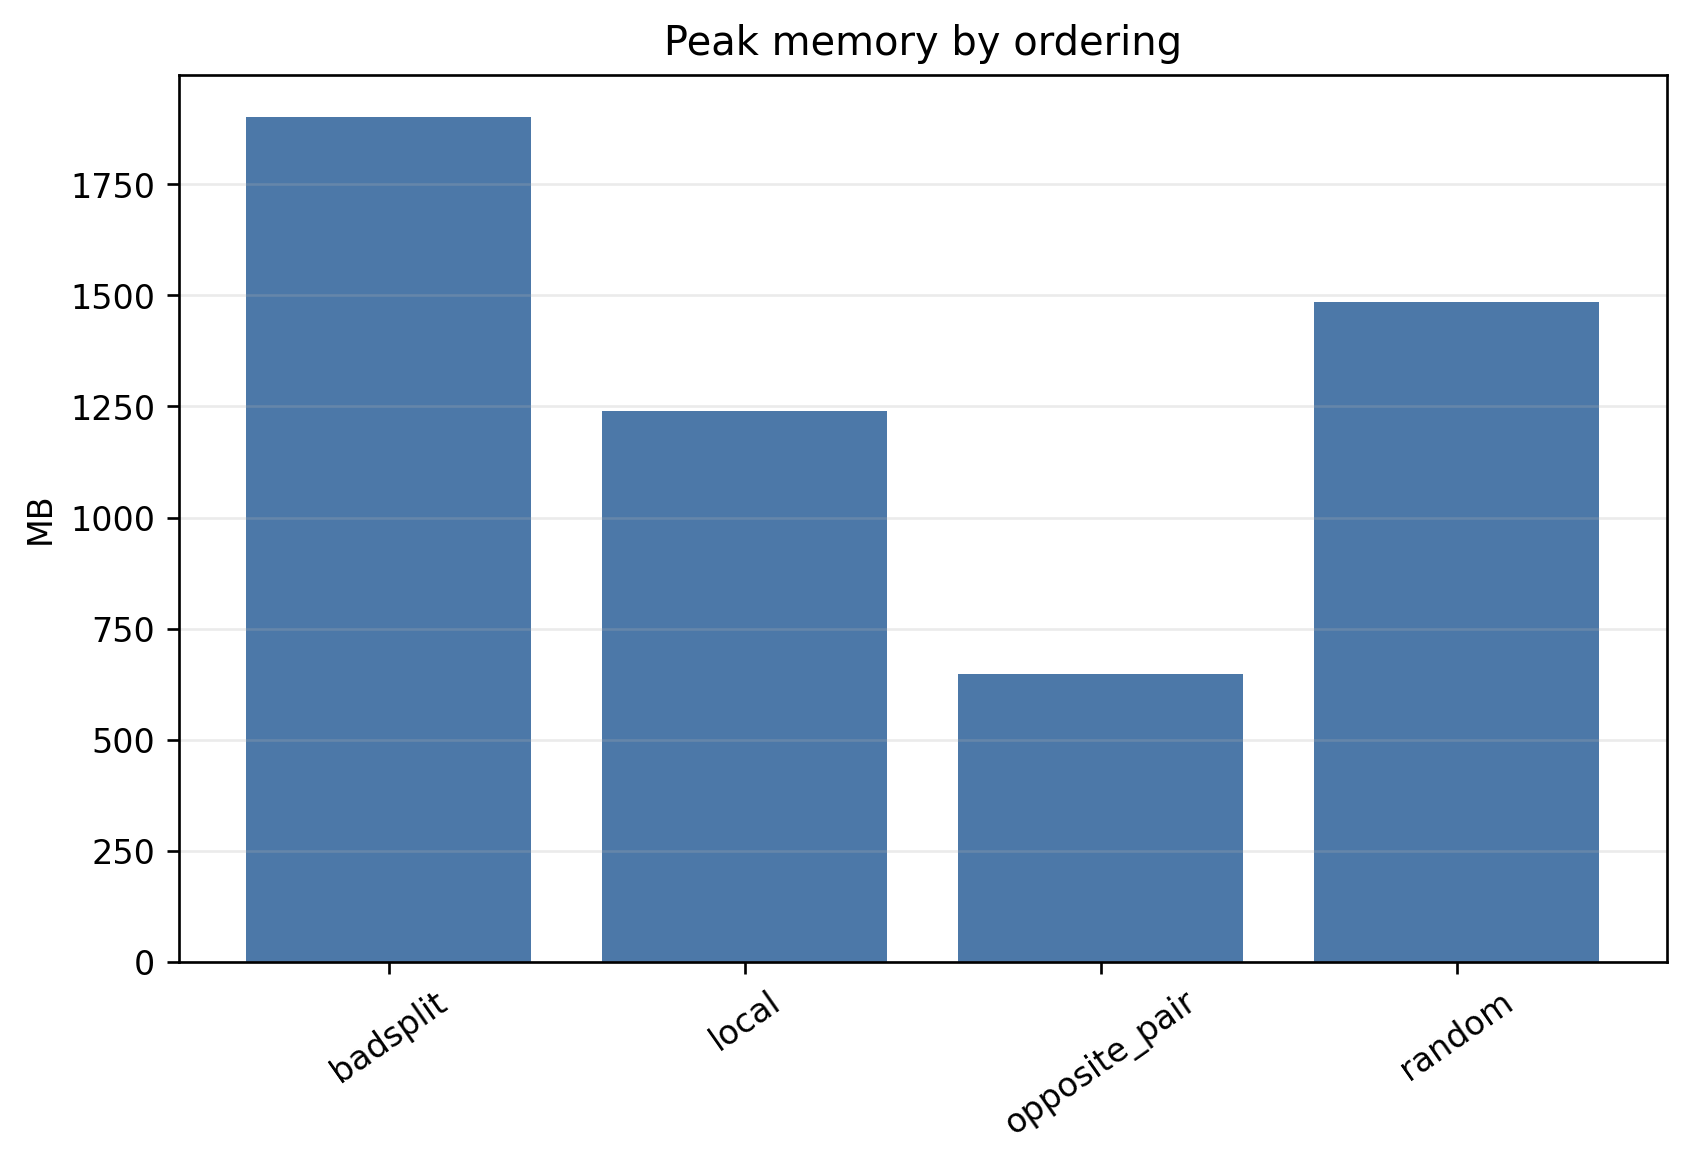
\includegraphics[width=0.72\linewidth]{peak_memory_vs_ordering.png}
  \caption{Peak memory by ordering. This figure is generated from
  repository diagnostics and should be regenerated after each experiment round.}
  \label{fig:peak-memory-ordering}
\end{figure}

\begin{figure}[t]
  \centering
  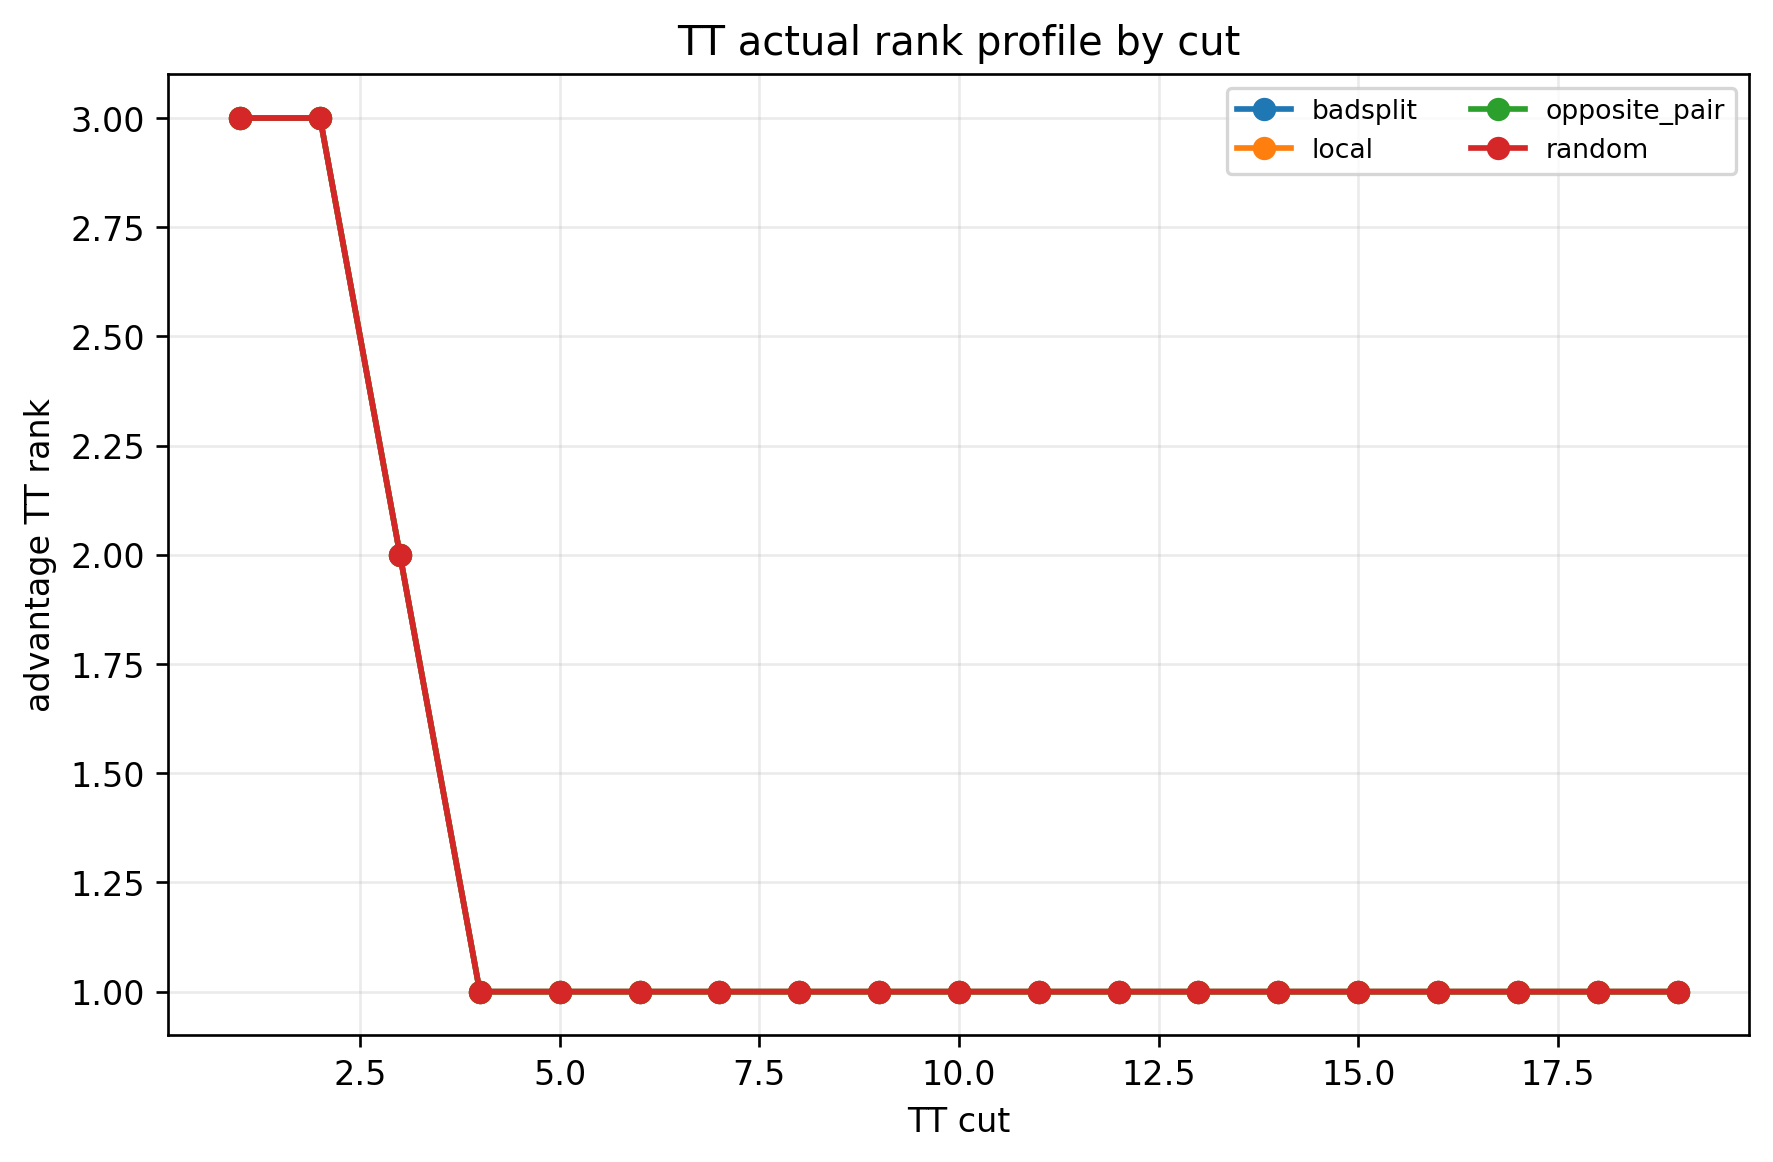
\includegraphics[width=0.72\linewidth]{tt_actual_rank_profile_by_ordering.png}
  \caption{Actual TT rank profile by ordering.}
  \label{fig:actual-rank-profile}
\end{figure}

\section{Conclusion}

The paper should conclude only after claims in \texttt{notes/claims.md} have
multi-seed evidence. Current smoke results validate the diagnostic path, not the
full performance claim.


\bibliographystyle{plainnat}
\bibliography{references}

\end{document}
